%!TEX root = abschlusspraesentation.tex

\begin{frame}[c]\frametitle{NN Auswertung}
\usetikzlibrary{arrows}
\usetikzlibrary{positioning} 
\usetikzlibrary{automata} 

  \def\wOne{{1.0,2.0,3.0,4.0}}
  \def\wTwo{{2.0,1.0,4.0,2.0,3.0,1.0}}

  \def\wOneAdjusted{{0.9,2.2,2.7,3.6}}
  \def\wTwoAdjusted{{3.0,0.5,3.7,1.8,2.5,0.5}}

  \def\inputValues{{0.3,0.2,0.5,0.6}}
  \def\results{{0.3,0.4,1.5,2.4}}
  \def\allresults{{-2.0, 4.6, 5.7, -3.0, 1.0, 4.4}}
  \def\allresultstransfered{{0.4, 0.8, 0.9, 0.3, 0.55, 0.8}}
  
  \def\rightresults{{0.3,0.4,1.5,2.4,2.0,2.0}}
  \def\allrightresults{{-5.7, 4.6, -5.7}}
  \def\allrightresultstransfered{{0.1, 0.8, 0.1}}
  \def\error{{-0.1, 0.2, -0.1}}
  \def\deltasoutput{{-0.0, 0.0, -0.0}}
  \def\deltashidden{{0.0, 0.0, 0.0, 0.0, 0.0, 0.0}}

  \begin{tikzpicture}[->,shorten >=1pt,auto, node distance=1cm, scale=0.9,
    thick,main node/.style={circle,fill=blue!20,draw,font=\sffamily\small\bfseries}]
    % =======
    % empty invisible node to avoid resize
    % =======
      \node at (-2,7) {};
    % =======
    % Input Neurons   
    % =======
    \only<1>{
      \foreach \x in {0, ..., 3} {
        \node[main node] (\x) at (0,5.8-1.2*\x) {};
      }
    }
    \only<2->{
      \foreach \x in {0, ..., 3} {
        \node[main node] (\x) at (0,5.8-1.2*\x) {$x_\x$};
      }
    }


    % =======
    % Hidden Neurons   
    % =======
    \only<1-3> {
      \foreach \x in {0, ..., 5} {
        \node[main node] (1\x) at (4,7-1.2*\x) {};
      }
    }
    \only<4> {
      \foreach \x in {0,2,3,4,5} {
        \node[main node] (1\x) at (4,7-1.2*\x) {};
      }
      \node[main node] (11) at (4,7-1.2) {$\sum\limits_{i=0}^3$};
    }
    \only<5> {
     \foreach \x in {0,2,3,4,5} {
        \node[main node] (1\x) at (4,7-1.2*\x) {};
      }
      \node[main node] (11) at (4,7-1.2) {$f\left(\sum\limits_{i=0}^3\right)$};
    }
     \only<6-13> {
      \foreach \x in {0,...,5} {
        \node[main node] (1\x) at (4,7-1.2*\x) {$y_\x$};
      }
    }
    \only<14-> {
      \foreach \x in {0,...,5} {
        \node[main node] (1\x) at (4,7-1.2*\x) {$\delta_{h\x}$};
      }
    }


    % =======
    % Output Neurons   
    % =======
    \only<1-7> {
      \foreach \x in {0, ..., 2} {
        \node[main node] (2\x) at (8,5.2-1.2*\x) {};
      }
    }
    \only<8> {
      \foreach \x in {0, 2} {
        \node[main node] (2\x) at (8,5.2-1.2*\x) {};
      }
       \node[main node] (21) at (8,5.2-1.2) {$\sum\limits_{i=0}^5$};
    }


     \only<9> {
      \foreach \x in {0, 2} {
        \node[main node] (2\x) at (8,5.2-1.2*\x) {};
      }
       \node[main node] (21) at (8,5.2-1.2) {$f\left(\sum\limits_{i=0}^5\right)$};
       
    }
     \only<10> {
      \foreach \x in {0,..., 2} {
        \node[main node] (2\x) at (8,5.2-1.2*\x) {$z_\x$};
      }
       
    }

    \only<11> {
      \foreach \x in {0,..., 2} {
          \node[main node] (2\x) at (8,5.2-1.2*\x) {$e_\x$};
      }
    }
    \only<12-> {
      \foreach \x in {0,..., 2} {
          \node[main node] (2\x) at (8,5.2-1.2*\x) {$\delta_\x$};
      }
    }

    
    


    
    % \ifthenelse{\iStepTwo>0 \and \iStepTwo<11}{
    %   \foreach \x in {0, ..., 3} {
    %     \node at (0.1*\iStepTwo,5.8-1.2*\x+\iStepTwo*\x*0.06) {\pgfmathparse{\inputValues[\x}\pgfmathresult};
    %   }
    % } 

    % \ifthenelse{\iStepThree>0 \and \iStepThree<11}{
    %   \foreach \x in {0, ..., 3} {
    %     \node [opacity=1.0-0.1*\iStepThree] at (1.0+0.08*\iStepThree,5.8-0.6*\x) {\pgfmathparse{\inputValues[\x}\pgfmathresult};
    %   }
    % } 

    % \ifthenelse{\iStepFour>0 \and \iStepFour<11}{
    %   \foreach \x in {0, ..., 3} {
    %     \node [opacity=0.1*\iStepFour] at (1.8,5.8-0.6*\x) {\pgfmathparse{\results[\x}\pgfmathresult};
    %   }
    % } 

    % \ifthenelse{\iStepFive>0 \and \iStepFive<11}{
    %   \foreach \x in {0, ..., 3} {
    %     \node at (1.8+0.2*\iStepFive,5.8-0.6*\x+0.06*\iStepFive*\x) {\pgfmathparse{\results[\x}\pgfmathresult};
    %   }
    % } 
    
    % =======
    % edges   
    % ======= 
    \only<1> {
      \foreach \x in {0, ..., 3} 
        \foreach \y in {0, ..., 5} {
          \ifthenelse{\y=1}{
            \path[every node/.style={font=\sffamily\small}]
              (\x) edge [opacity=0.5] node [left] {} (1\y);
          }{
            \path[every node/.style={font=\sffamily\small}]
              (\x) edge [opacity=0.2] node [left] {} (1\y);
          }
        }
      
      \foreach \x in {0, ..., 5} 
        \foreach \y in {0, ..., 2} {
          \ifthenelse{\y=1}{
            \path[every node/.style={font=\sffamily\small}]
              (1\x) edge [opacity=0.5] node [left] {} (2\y);
          }{
            \path[every node/.style={font=\sffamily\small}]
              (1\x) edge [opacity=0.2] node [left] {} (2\y);
          }
        }
    }
    
    \only<2> {
      \foreach \x in {0, ..., 3} 
        \foreach \y in {0, ..., 5} {
          \ifthenelse{\y=1}{
            \path[every node/.style={font=\sffamily\small}]
              (\x) edge [opacity=0.5] node [left, sloped, above, opacity=1.0] {$v_{\x}$} (1\y);
          }
        }
      
      \foreach \x in {0, ..., 5} 
        \foreach \y in {0, ..., 2} {
          \ifthenelse{\y=1}{
            \path[every node/.style={font=\sffamily\small}]
              (1\x) edge [opacity=0.5] node [left, sloped, above, opacity=1.0] {$w_{\x}$} (2\y);
          }
        }
    }

    \only<3> {
      \foreach \x in {0, ..., 3} 
        \foreach \y in {0, ..., 5} {
          \ifthenelse{\y=1}{
            \path[every node/.style={font=\sffamily\small}]
              (\x) edge [opacity=0.5] node [left, sloped, above, opacity=1.0, pos=0.4] {$v_{\x}\cdot x_\x$} (1\y);
          }
        }
      
      \foreach \x in {0, ..., 5} 
        \foreach \y in {0, ..., 2} {
          \ifthenelse{\y=1}{
            \path[every node/.style={font=\sffamily\small}]
              (1\x) edge [opacity=0.5] node [left, sloped, above, opacity=1.0] {$w_{\x}$} (2\y);
          }
        }
    }

    \only<4-6> {
      \foreach \x in {0, ..., 3} 
        \foreach \y in {0, ..., 5} {
          \ifthenelse{\y=1}{
            \path[every node/.style={font=\sffamily\small}]
              (\x) edge [opacity=0.5] node [left, sloped, above, opacity=1.0, pos=0.4] {$v_{\x}$} (1\y);
          }
        }
      
      \foreach \x in {0, ..., 5} 
        \foreach \y in {0, ..., 2} {
          \ifthenelse{\y=1}{
            \path[every node/.style={font=\sffamily\small}]
              (1\x) edge [opacity=0.5] node [left, sloped, above, opacity=1.0] {$w_{\x}$} (2\y);
          }
        }
    }
    \only<7> {
      \foreach \x in {0, ..., 3} 
        \foreach \y in {0, ..., 5} {
          \ifthenelse{\y=1}{
            \path[every node/.style={font=\sffamily\small}]
              (\x) edge [opacity=0.5] node [left, sloped, above, opacity=1.0, pos=0.4] {$v_{\x}$} (1\y);
          }
        }
      
      \foreach \x in {0, ..., 5} 
        \foreach \y in {0, ..., 2} {
          \ifthenelse{\y=1}{
            \path[every node/.style={font=\sffamily\small}]
              (1\x) edge [opacity=0.5] node [left, sloped, above, opacity=1.0, pos=0.4] {$w_{\x}\cdot y_\x$} (2\y);
          }
        }
    }
    \only<8-12> {
      \foreach \x in {0, ..., 3} 
        \foreach \y in {0, ..., 5} {
          \ifthenelse{\y=1}{
            \path[every node/.style={font=\sffamily\small}]
              (\x) edge [opacity=0.5] node [left, sloped, above, opacity=1.0, pos=0.4] {$v_{\x}$} (1\y);
          }
        }
      
      \foreach \x in {0, ..., 5} 
        \foreach \y in {0, ..., 2} {
          \ifthenelse{\y=1}{
            \path[every node/.style={font=\sffamily\small}]
              (1\x) edge [opacity=0.5] node [left, sloped, above, opacity=1.0] {$w_{\x}$} (2\y);
          }
        }
    }
    \only<13> {
      \foreach \x in {0, ..., 3} 
        \foreach \y in {0, ..., 5} {
          \ifthenelse{\y=1}{
            \path[every node/.style={font=\sffamily\small}]
              (\x) edge [opacity=0.5] node [left, sloped, above, opacity=1.0, pos=0.4] {$v_{\x}$} (1\y);
          }
        }
      
      \foreach \x in {0, ..., 5} 
        \foreach \y in {0, ..., 2} {
          \ifthenelse{\y=1}{
            \path[every node/.style={font=\sffamily\small}]
              (1\x) edge [opacity=0.5] node [left, sloped, above, opacity=1.0] {$w^*_{\x}$} (2\y);
          }
        }
    }
     \only<14> {
      \foreach \x in {0, ..., 3} 
        \foreach \y in {0, ..., 5} {
          \ifthenelse{\y=1}{
            \path[every node/.style={font=\sffamily\small}]
              (\x) edge [opacity=0.5] node [left, sloped, above, opacity=1.0, pos=0.4] {$v_{\x}$} (1\y);
          }
        }
      
      \foreach \x in {0, ..., 5} 
        \foreach \y in {0, ..., 2} {
          \ifthenelse{\y=1}{
            \path[every node/.style={font=\sffamily\small}]
            (1\x) edge [opacity=0.5] node [left, sloped, above, opacity=1.0] {$w^*_\x$} (2\y);
          }
        }
    }
    \only<15-> {
      \foreach \x in {0, ..., 3} 
        \foreach \y in {0, ..., 5} {
          \ifthenelse{\y=1}{
            \path[every node/.style={font=\sffamily\small}]
              (\x) edge [opacity=0.5] node [left, sloped, above, opacity=1.0, pos=0.4] {$v^*_{\x}$} (1\y);
          }
        }
      
      \foreach \x in {0, ..., 5} 
        \foreach \y in {0, ..., 2} {
          \ifthenelse{\y=1}{
            \path[every node/.style={font=\sffamily\small}]
              (1\x) edge [opacity=0.5] node [left, sloped, above, opacity=1.0] {$w^*_{\x}$} (2\y);
          }
        }
    }
   \end{tikzpicture}
  \begin{itemize}
    \only<1> {
      \item Multilayerperceptron-Netz
    }
    \only<2> {
      \item Trainingseingabe und Kantengewichte
    }
    \only<3> {
      \item Gewichtung der Trainingseingabe mit Kantengewicht
    }
    \only<4> {
      \item Summe der Produkte ergibt Netzeingabe in der Hidden-Schicht
    }
    \only<5> {
      \item Netzeingabe der restlichen Neuronen der Hidden-Schicht
    }
    \only<6> {
      \item Umrechnung der Netzeingabe mit der Übertragungsfunktion (sigmoiddelta)
    }
    \only<7> {
      \item Gewichtung der Ausgabewerte mit Kantengewicht
    }
    \only<8> {
      \item Summe der Produkte ergibt Netzeingabe in der Ausgabeschicht
    }
    \only<9> {
      \item Netzeingabe der restlichen Neuronen der Ausgabeschicht
    }
    \only<10> {
      \item Umrechnung der Netzeingabe mit der Übertragungsfunktion (sigmoiddelta)
    }
    \only<11> {
      \item Berechnung des Ausgabefehlers anhand Ausgabewert und gewünschtem Ausgabewert
    }
    \only<12> {
      \item Berechnung von delta-Werten anhand Netzeingabe, Übertragungsfunktion und Ausgabefehler 
    }
    \only<13> {
      \item Anpassung der Kantengewichte
    }
    \only<14> {
      \item Berechnung von delta-Werten in Hidden-Schicht (benötigt u.a. ausgehende Kantengewichte und delta-Werte der Ausgabeschicht)
    }
    \only<15> {
      \item Anpassung der Kantengewichte
    }
   \end{itemize}
  
% \item<1> Multilayerperceptron-Netz
%       \item<2> Trainingseingabe und Kantengewichte
%       \item<3> Gewichtung der Trainingseingabe mit Kantengewicht
%       \item<4> Summe der Produkte ergibt Netzeingabe in der Hidden-Schicht
%       \item<5> Netzeingabe der restlichen Neuronen der Hidden-Schicht
%       \item<6> Umrechnung der Netzeingabe mit der Übertragungsfunktion (sigmoiddelta)
%       \item<7> Gewichtung der Ausgabewerte mit Kantengewicht
%       \item<8> Summe der Produkte ergibt Netzeingabe in der Output-Schicht
%       \item<9> Netzeingabe der restlichen Neuronen der Output-Schicht
%       \item<10> Umrechnung der Netzeingabe mit der Übertragungsfunktion (sigmoiddelta)
%       \item<11> b
%       \item<12> Berechnung von delta-Werten anhand Netzeingabe, Übertragungsfunktion und Ausgabefehler 
%       \item<13> b

    % \node[main node] (0) {5};
    % \node[main node] (1) [below of=0] {\only<2>{test}};
    % \node[main node] (2) [below of=1] {3};
    % \node[main node] (3) [below of=2] {4};

    % \node[main node] (11) [right of=0] {2};
    % \node[main node] (10) [above of=11] {2};
    % \node[main node] (12) [right of=1] {2};
    % \node[main node] (13) [right of=2] {2};
    % \node[main node] (14) [right of=3] {2};
    % \node[main node] (15) [below of=14] {2};

    % \node[main node] (20) [below right  of=10] {2};
    % \node[main node] (21) [below right  of=12] {2};
    % \node[main node] (22) [below right  of=14] {2};

    % \path[every node/.style={font=\sffamily\small}]
    %   (0) edge node [left] {0.6} (10)
    %       edge node[left] {0.3} (11)
    %       edge node {0.1} (12)
    %   (1) edge node [right] {0.4} (10)
    %       edge node {0.3} (11)
    %       edge node {0.4} (12)
    %       edge node {0.1} (13)
    %   (2) edge node [right] {0.8} (13)
    %       edge node [right] {0.2} (14)
    %       edge node [right] {0.2} (15)
    %   (3) edge node [left] {0.2} (15)

    %   (10)edge node [left] {0.6} (20)
    %   (11)edge node [right] {0.4} (20)
    %       edge node {0.3} (21)
    %       edge node {0.4} (22)
    %   (12)edge node [right] {0.8} (21)
    %       edge node [right] {0.2} (20)
    %   (13)edge node [left] {0.2} (20)
    %   (14)edge node [right] {0.8} (21)
    %       edge node [right] {0.2} (22)
    %   ;
    
\end{frame}
